%!TEX root=/home/ska124/Dropbox/Thesis/thes-full.tex

%%%%%%%%%%%%%%%%%%%%%%%%%%%%%%%%%%%%%%%%%%%%%%%%%
%
%     Chapter 5
%
%%%%%%%%%%%%%%%%%%%%%%%%%%%%%%%%%%%%%%%%%%%%%%%%

\chapter{Evaluation}
\label{chap:evaluation}
This chapter evaluates the performance of the \AC\ described in Chapter~\ref{chap:ac_architecture}. The evaluation is performed using the infrastructure described in Chapter~\ref{sec:simulation_infrastructure}. This chapter is divided into sections based on performance evaluations of:
\begin{itemize}[noitemsep]
	\item Comparison against a fixed granularity cache
	\item Adaptivity of the \AC\
	\item The spatial pattern predictor
	\item \AC\ versus other approaches
\end{itemize}

\section{Improved Memory Hierarchy Efficiency}
\label{sec:efficiency}
\vspace{5pt}
\noindent \textbf{Result 1:}{\emph~{\AC\ increases cache capacity by harvesting
  space from unused words and can achieve an 18\% reduction in both L1 and
  L2 miss rate.}
\\ \\
\noindent \textbf{Result 2:}{\emph~{\AC\ adaptively sizes the cache block
  granularity and reduces L1$\leftrightarrow$L2 bandwidth by 46\% and
  L2$\leftrightarrow$Memory bandwidth by 38\%.}
}
\\ \\
In this section, the bandwidth and miss rate properties of an \AC\ are compared against a conventional cache. A \textit{Fixed} cache represents a conventional cache which allocates a fixed granularity cache block on a refill request. The accuracy of the spatial pattern predictor is an important factor which governs the accuracy of the \AC\ and is evaluated separately. For the results presented in this section, cache line utilisation statistics, gathered from a prior run of the application on a conventional cache, are used to drive the predictor. This isolates the benefits of the \AC\ from the potentially changing accuracy of the spatial pattern predictor across different cache geometries. This also ensures that the spatial granularity predictions can be replayed across multiple simulation runs. To ensure equivalent data storage space, the \AC\ size is set to the sum of the tag array and the data array in a conventional cache. At the L1 level (64K), the net capacity of the \AC\ is 64K + 8*4*256 bytes and at the L2 level (1M) configuration, it is 1M + 8*8*2048 bytes. The L1 cache has 256 sets and the L2 cache has 2048 sets. 

Fig~\ref{fig:eval_scatter_bw_64k_1m} plots the miss rate and the traffic characteristics of the \AC{}.  Since \AC{} can hold blocks varying in size from 8B to 64B, each set can hold more blocks by utilizing the space saved from eliminating untouched words. The \AC\ reduces the 64K L1 miss rate on average by 23\%\footnote{All reported averages are geometric mean unless otherwise specified.} and standard deviation(SD) of 24 for the Low group, and by 21\%(SD:16) for the moderate group; even applications with high spatial locality experience a 7\%(SD:8) improvement in miss rate. There is a 46\%(SD:20) reduction on average in L1$\leftrightarrow$L2 bandwidth. At the 1M L2 level, the \AC\ improves the moderate group's miss rate by 8\%(SD:10) and bandwidth by 23\%(SD:12).  Applications with moderate utilization make better use of the space harvested from unused words by \AC{}. Many low utilization applications tend to be streaming and providing extra cache space does not help lower miss rate. However, by not fetching unused words, the \AC\ achieves a significant reduction (38\%(SD:24) on average) in off-chip L2$\leftrightarrow$Memory bandwidth; even High utilization applications see a 17\%(SD:15) reduction in bandwidth.  Utilization and miss rate are not, however, always directly correlated (more details in \S~\ref{sec:adaptivity}).

With the \AC\, the number of blocks per set varies based on the granularity of the blocks being fetched, which in turn depends on the spatial locality in the application. Table~\ref{table:blockcount} shows the average number of blocks per set. In applications with low spatial locality, the \AC\ adjusts the block size and adapts to store many smaller blocks. The 64K L1 \AC\ stores 10 blocks per set for mcf and 12 blocks per set for art, effectively increasing associativity without introducing hardware overheads. At the L2, when the working set starts to fit in the L2 cache, the set is partitioned into fewer blocks. 

\begin{figure}[ht]

  \subfloat[64K - Low]{
    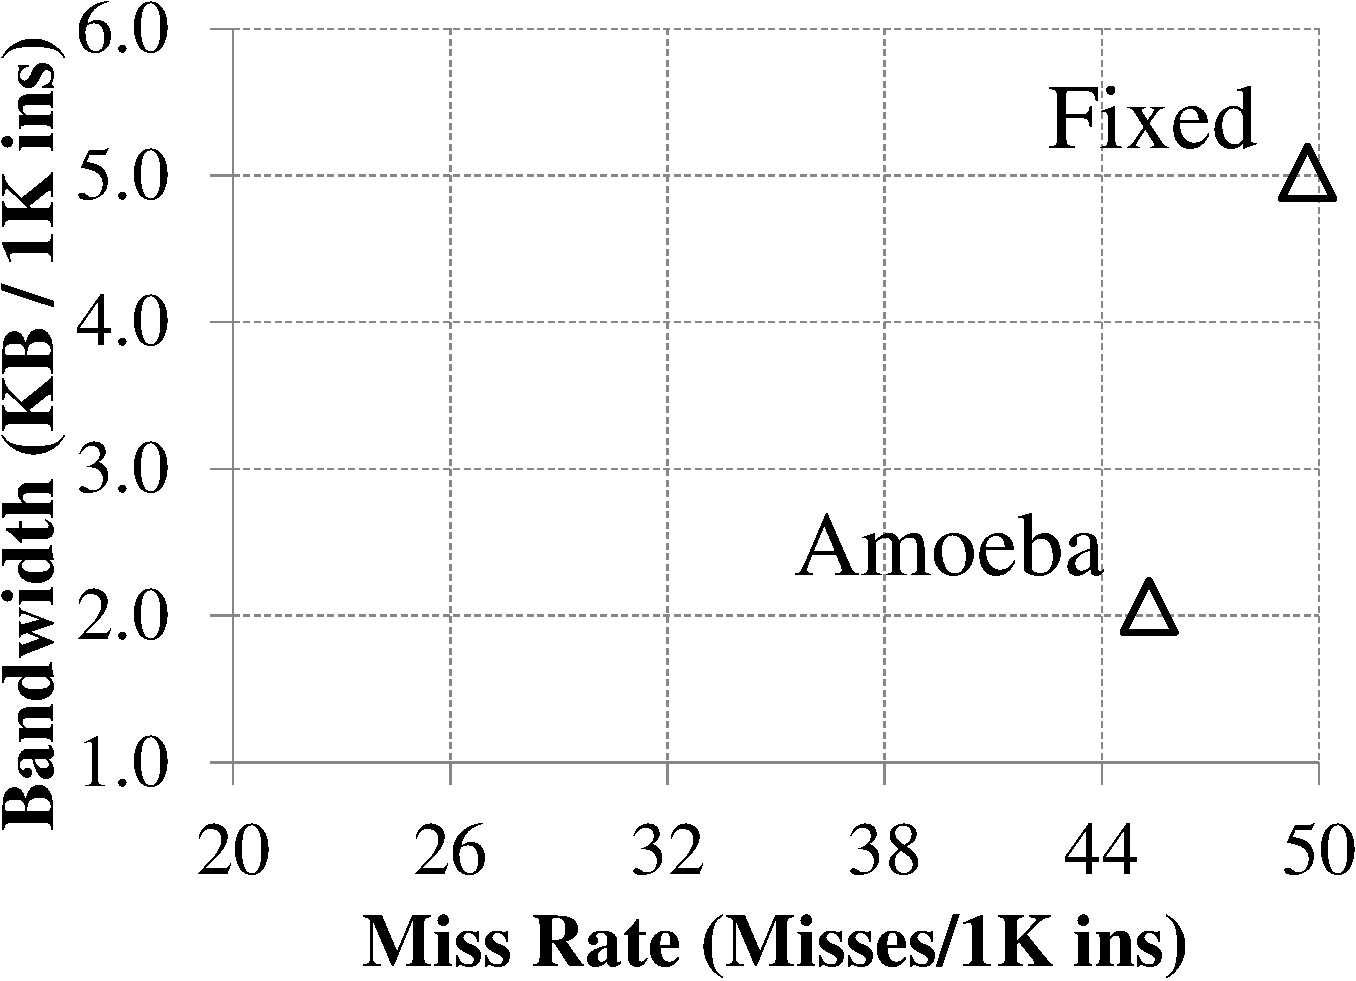
\includegraphics[width=0.48\textwidth]{files/Plots/08-Scatter_Bw_Miss_64K_low.pdf}
  }
  \subfloat[1M - Low]{
     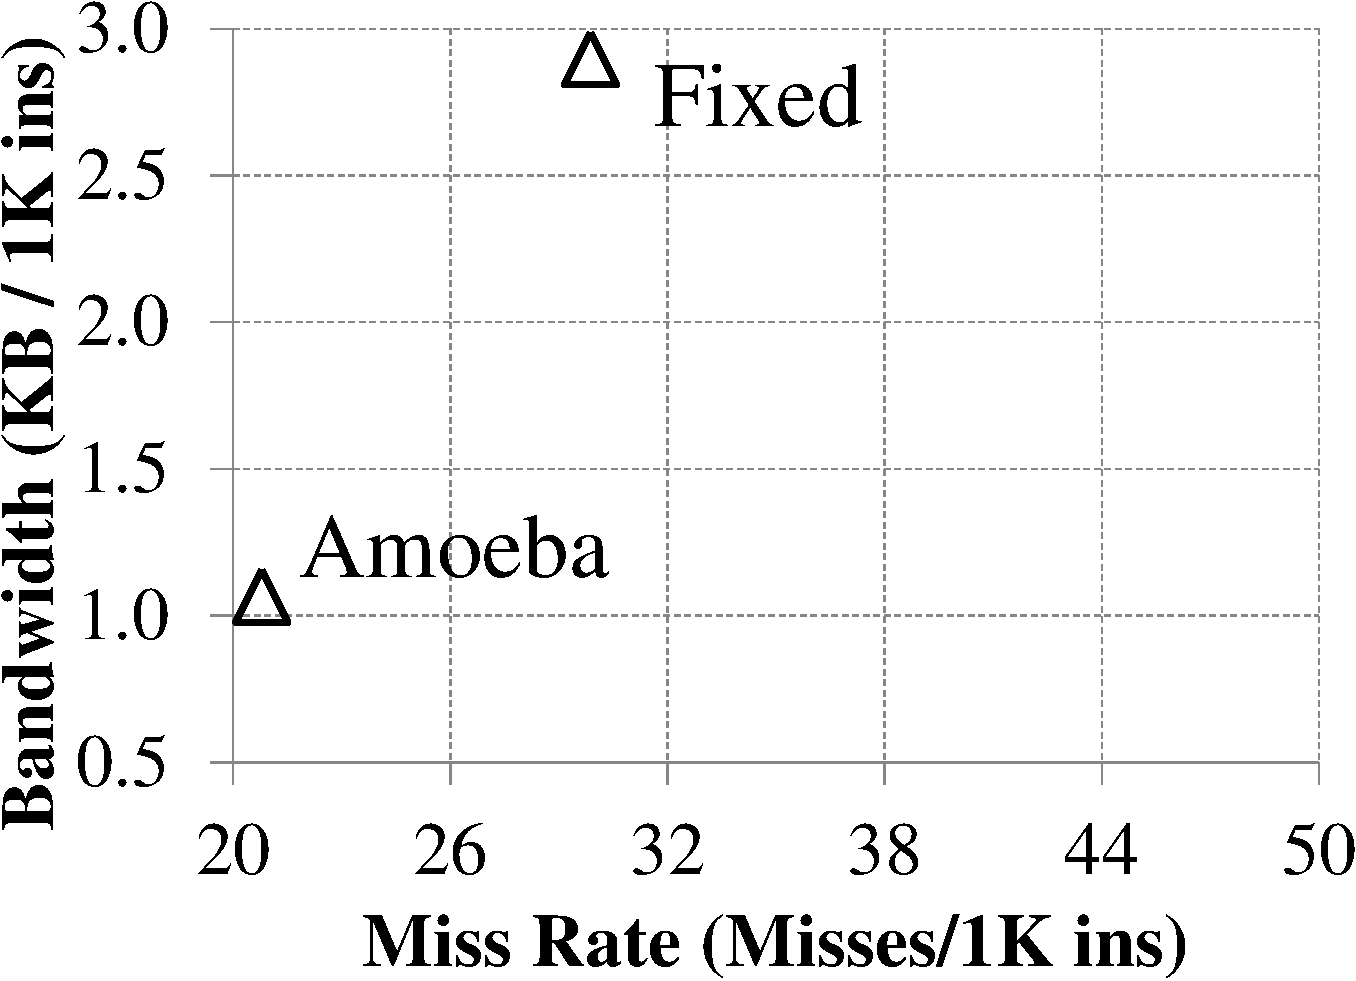
\includegraphics[width=0.48\textwidth]{files/Plots/08-Scatter_Bw_Miss_1M_low.pdf}
  }
  
  \subfloat[64K - Moderate]{
    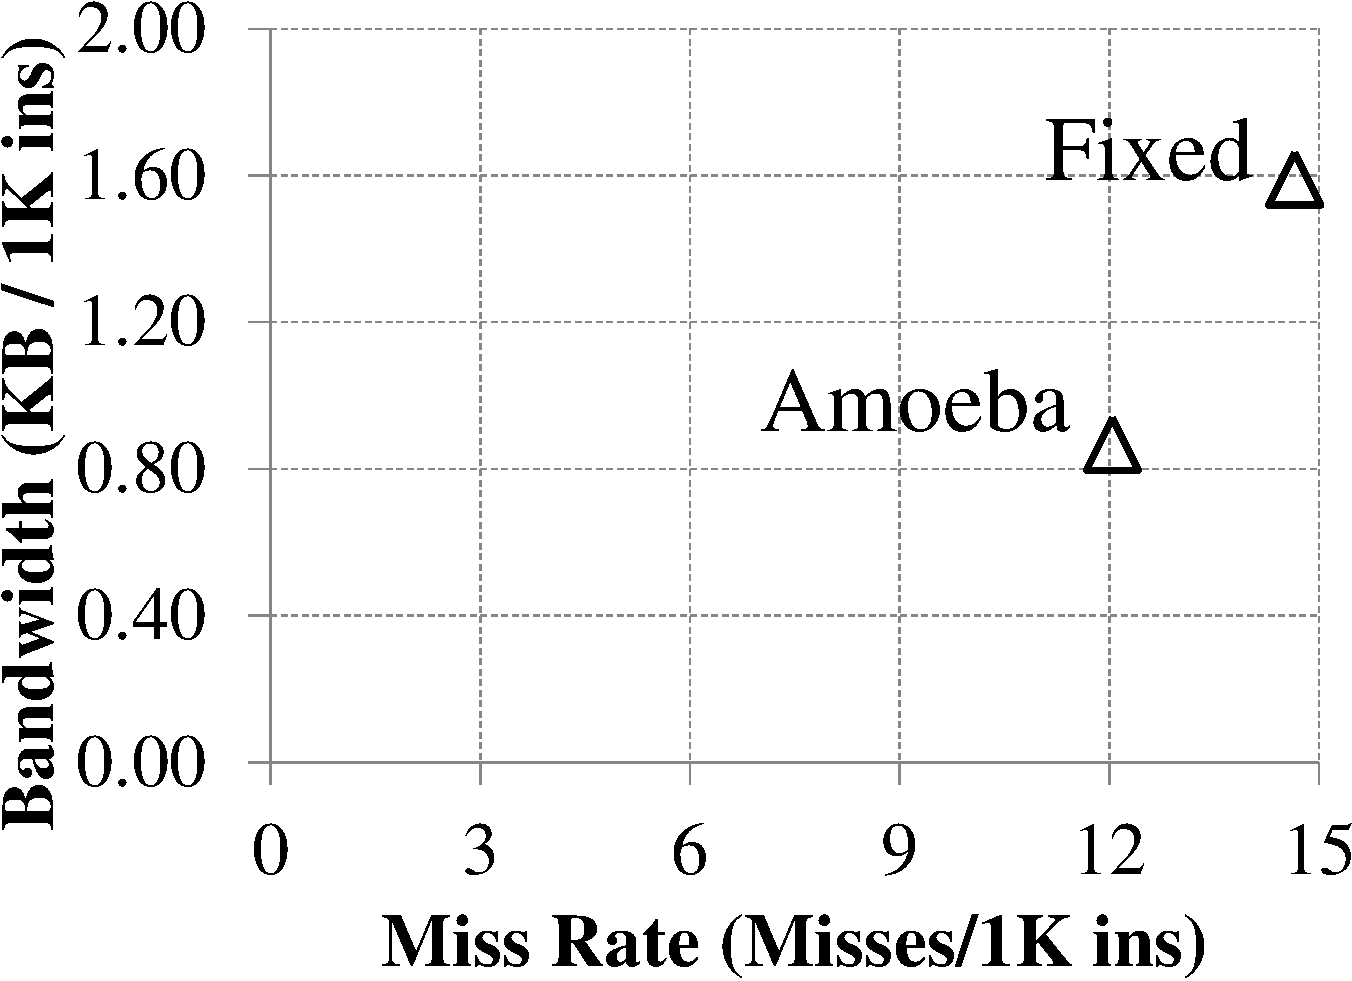
\includegraphics[width=0.48\textwidth]{files/Plots/08-Scatter_Bw_Miss_64K_mod.pdf}
  }
  \subfloat[1M - Moderate]{
     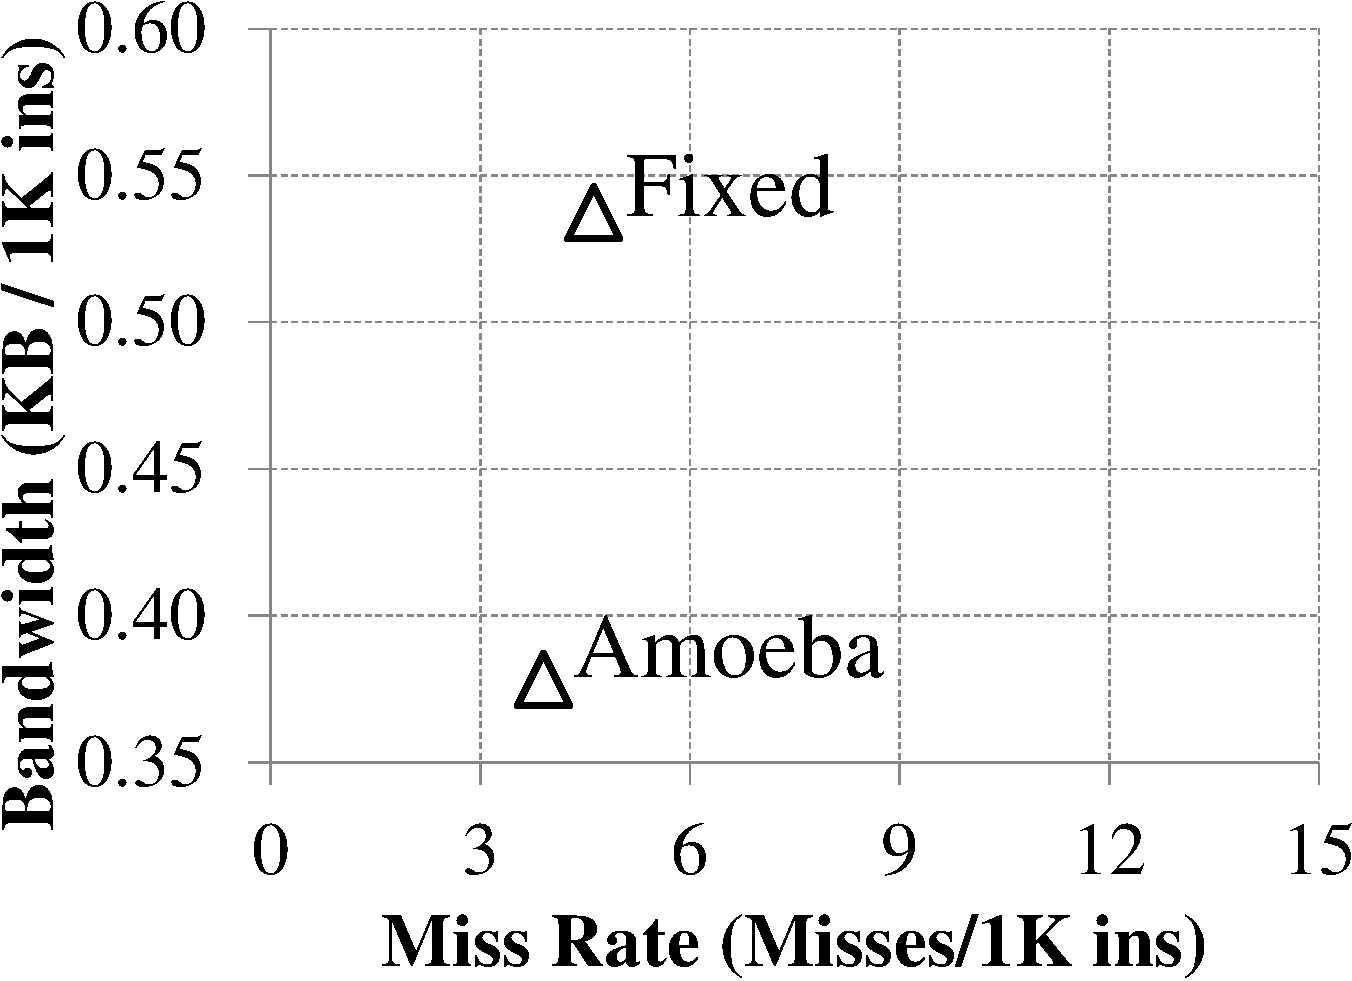
\includegraphics[width=0.48\textwidth]{files/Plots/08-Scatter_Bw_Miss_1M_mod.pdf}
  }
    
  \subfloat[64K - High]{
    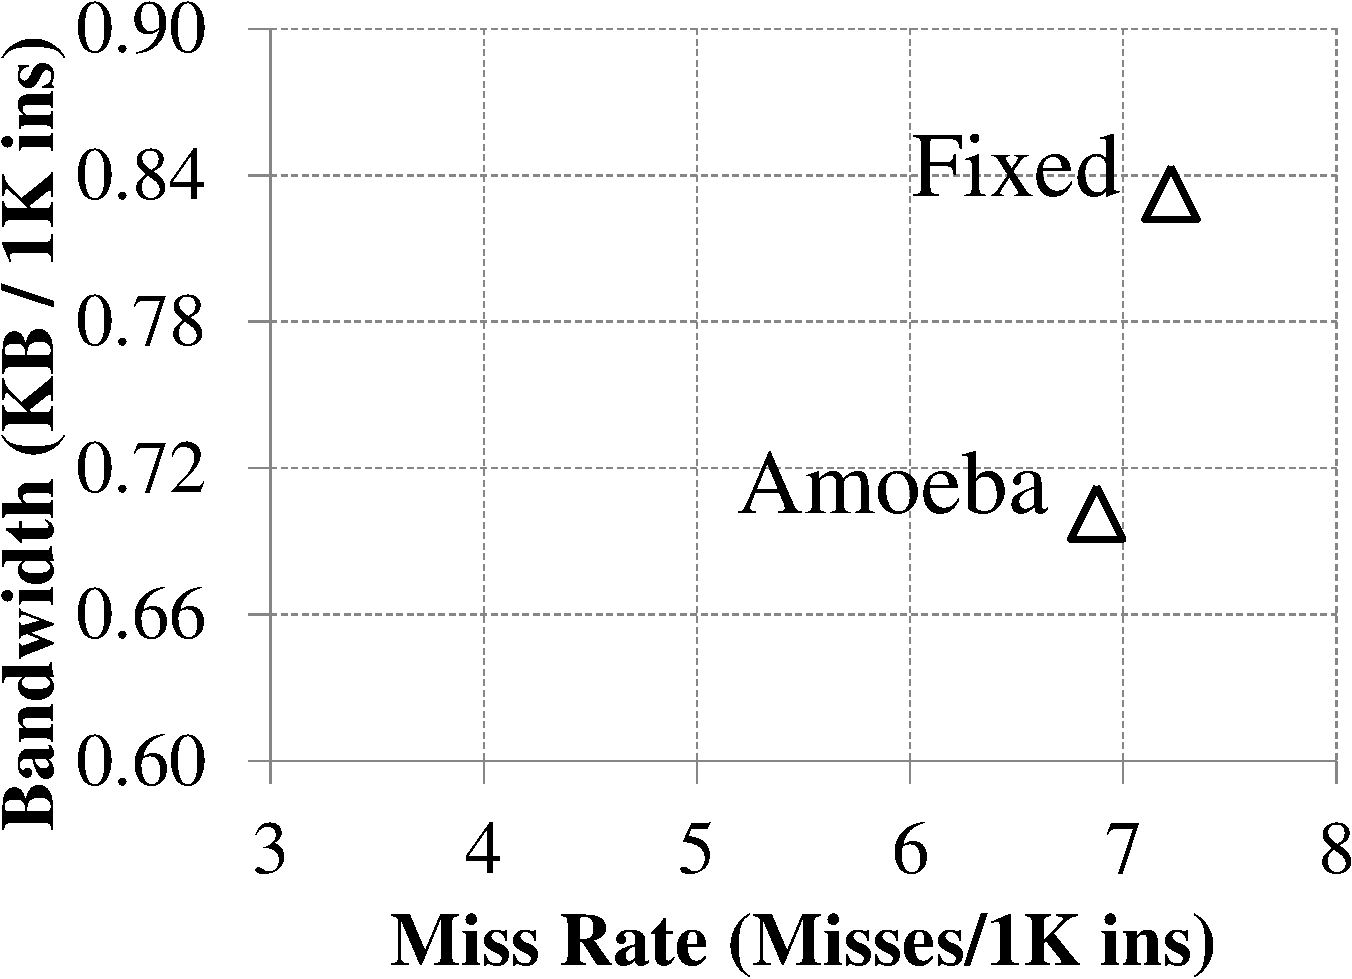
\includegraphics[width=0.48\textwidth]{files/Plots/08-Scatter_Bw_Miss_64K_high.pdf}
  }
  \subfloat[1M - High]{
     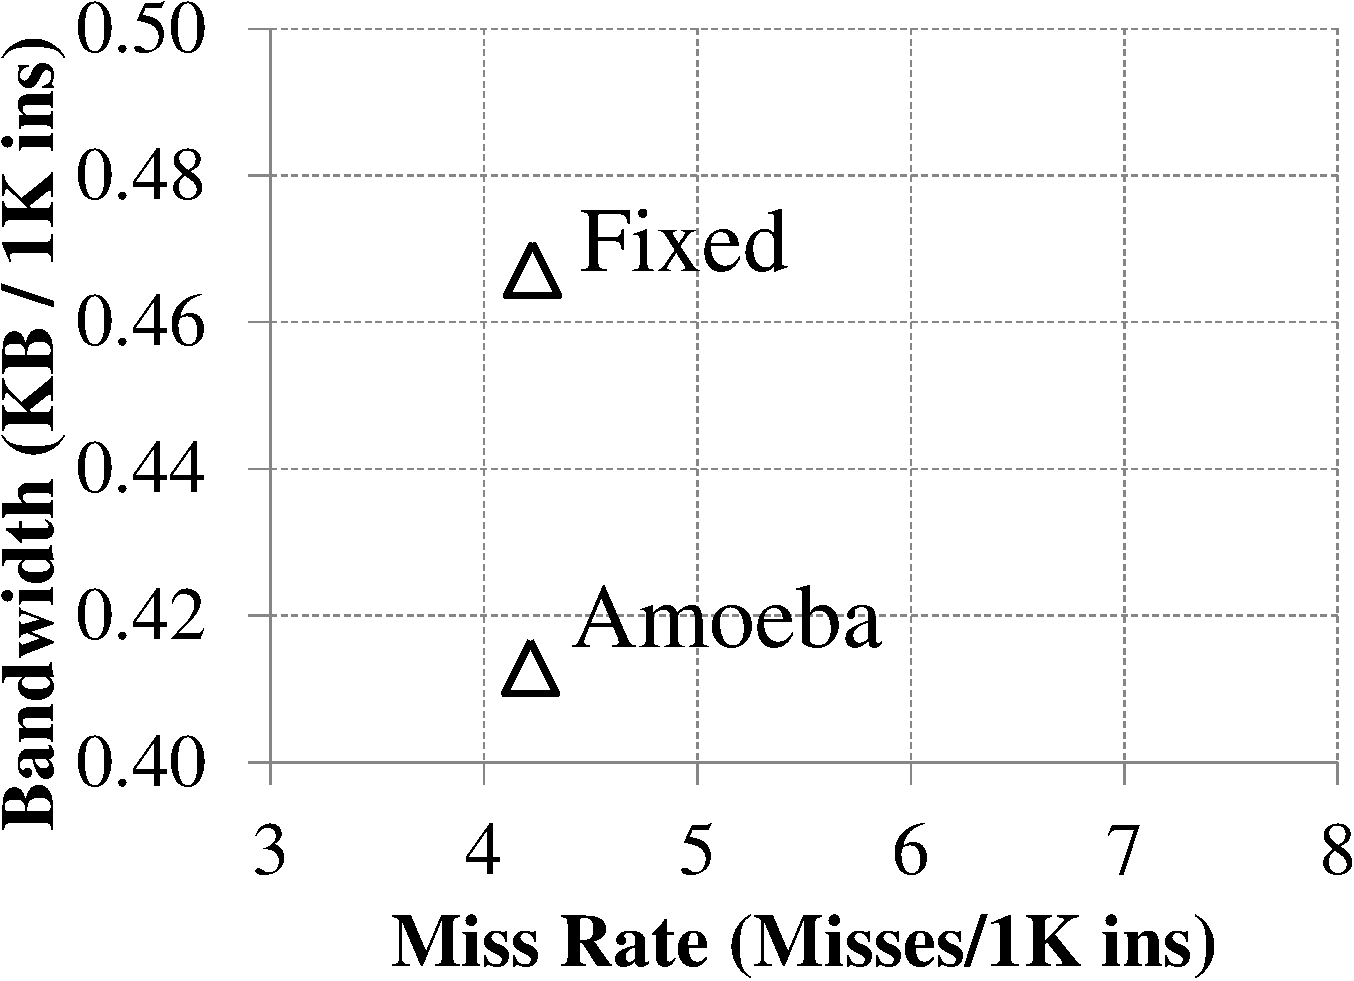
\includegraphics[width=0.48\textwidth]{files/Plots/08-Scatter_Bw_Miss_1M_high.pdf}
  }

  \caption[Bandwidth vs. Miss Rate]{Bandwidth vs. Miss Rate for a fixed granularity cache and \AC{}. (a),(c),(e): 64K, 4-wayL1 equivalent (b),(d),(f): 1M, 8-way LLC equivalent.  Markers on the plot indicate cache block size. Note the different scales for different groups.}
  \label{fig:eval_scatter_bw_64k_1m}
\end{figure}

\clearpage

%!TEX root=/home/ska124/Dropbox/Thesis/thes-full.tex
\begin{table}[h]
  \centering
  \begin{tabular}{|c|c|}
  \hline 
    Blocks/Set & 64K Cache, 288 B/set \\
    \hline
    4---5  &  ferret, cactus, firefox, eclipse, facesim, freqmine, milc, astar\\
    6---7  &  tpc-c, tradesoap, soplex, apache, fluidanimate\\
    8---9  &  h2, canneal, omnetpp, twolf, x264, lbm, jbb \\
    10---12 & mcf, art \\
    \hline
    \multicolumn{2}{c}{} \\
    \hline
    Blocks/Set & 1M Cache, 576 B/set \\
    \hline
    3---5 & eclipse, omnetpp   \\
    8---9 & cactus, firefox, tradesoap, freqmine, h2, x264, tpc-c   \\
    10---11  & facesim, soplex, astar, milc, apache, ferret  \\
    12---13  & twolf, art, jbb, lbm , fluidanimate \\
    15---18 & canneal, mcf \\
    \hline
  \end{tabular}
  \caption[Amoeba Blocks per set]{Average number of \AB{}s per set}
  \label{table:blockcount}
\end{table}


Note that applications like eclipse and omnetpp hold only 3---5 blocks per set on average (lower than conventional associativity) due to their low miss rates (see Table~\ref{table:Abs_Eval_Oracle}). With streaming applications (e.g., canneal), \AC\ increases the number of blocks/set to $>$15 on average. Finally, some applications like apache store between 6---7 blocks/set with a 64K cache with varied block sizes (see Figure~\ref{fig:StackBar_PredictorSize}): approximately 50\% of the blocks store 1-2 words and 30\% of the blocks store 8 words at the L1. As the size of the cache increases and thereby the lifetime of the blocks, the \AC\ adapts to store larger size blocks as can be seen in Figure~\ref{fig:StackBar_PredictorSize}.
\\ \\
\indent Utilization is improved greatly across all applications (90\%+ in many cases). Figure~\ref{fig:StackBar_PredictorSize} shows the distribution of cache block granularities in \AC{}. The \AB\ distribution matches the word access distribution presented in Fig~\ref{fig:stackbar_words_64k}). With the 1M cache, the larger cache size improves block lifespan and thereby utilization, with a significant drop in the \% of 1---2 word blocks. However, in many applications (tpc-c, apache, firefox, twolf, lbm, mcf), up to 20\% of the blocks are 3--6 words wide, indicating the benefits of adaptivity and the challenges faced by a fixed granularity conventional cache.

\begin{figure}[!h]
  \centering
  \subfloat[64K L1 cache]{
    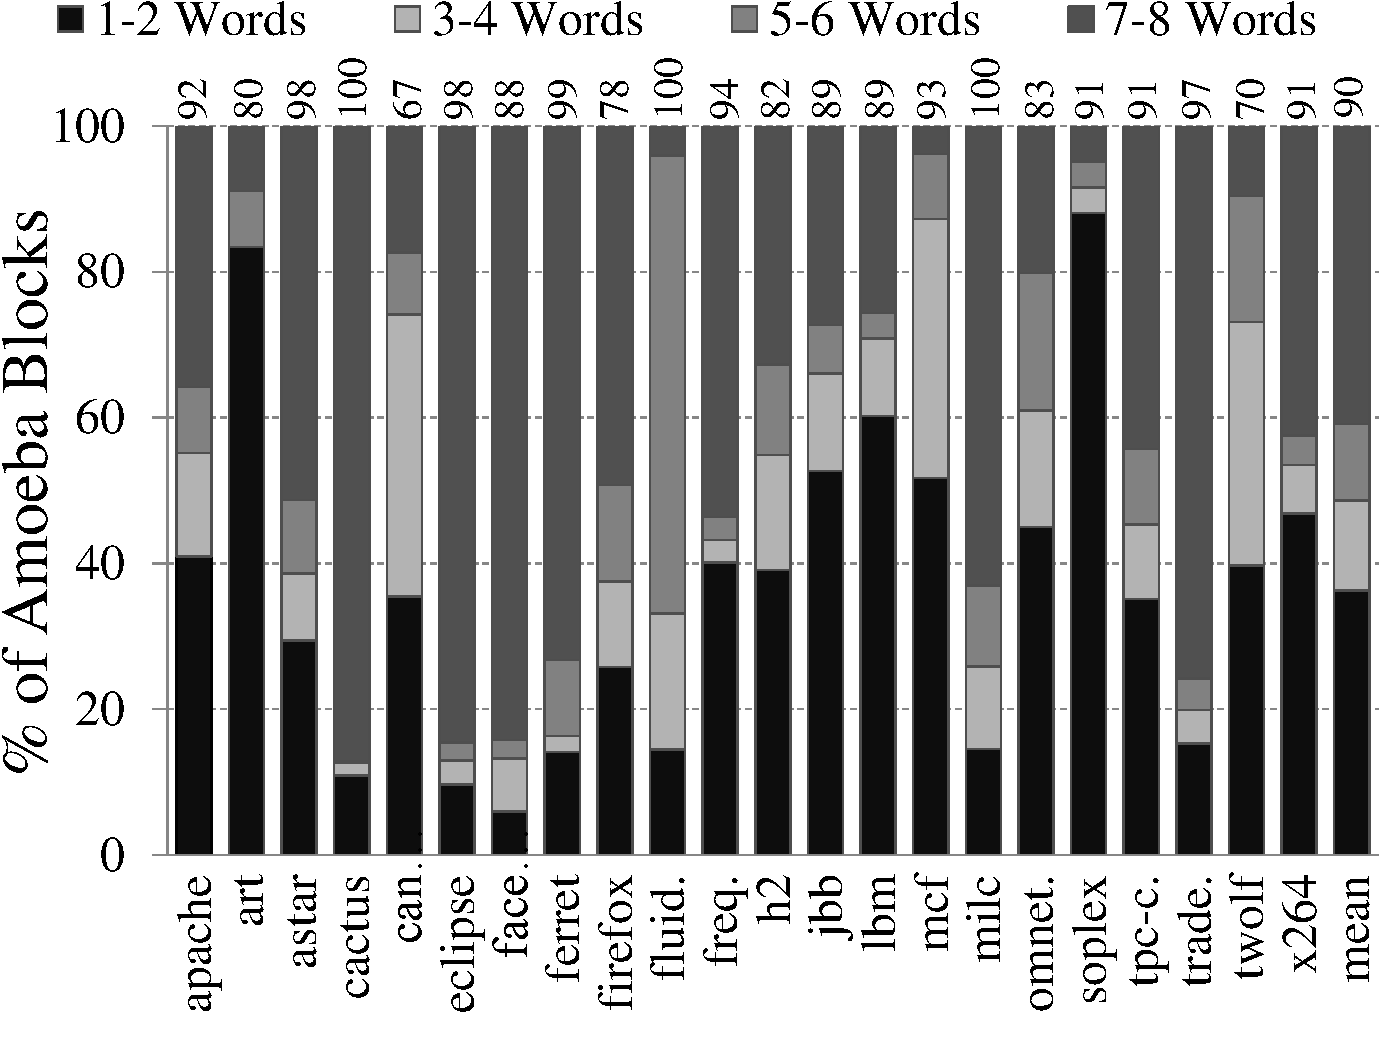
\includegraphics[width=0.8\textwidth]{files/Plots/08-StackBar_PredictSize_64K.pdf}
  }

  \subfloat[1M L2 cache]{
    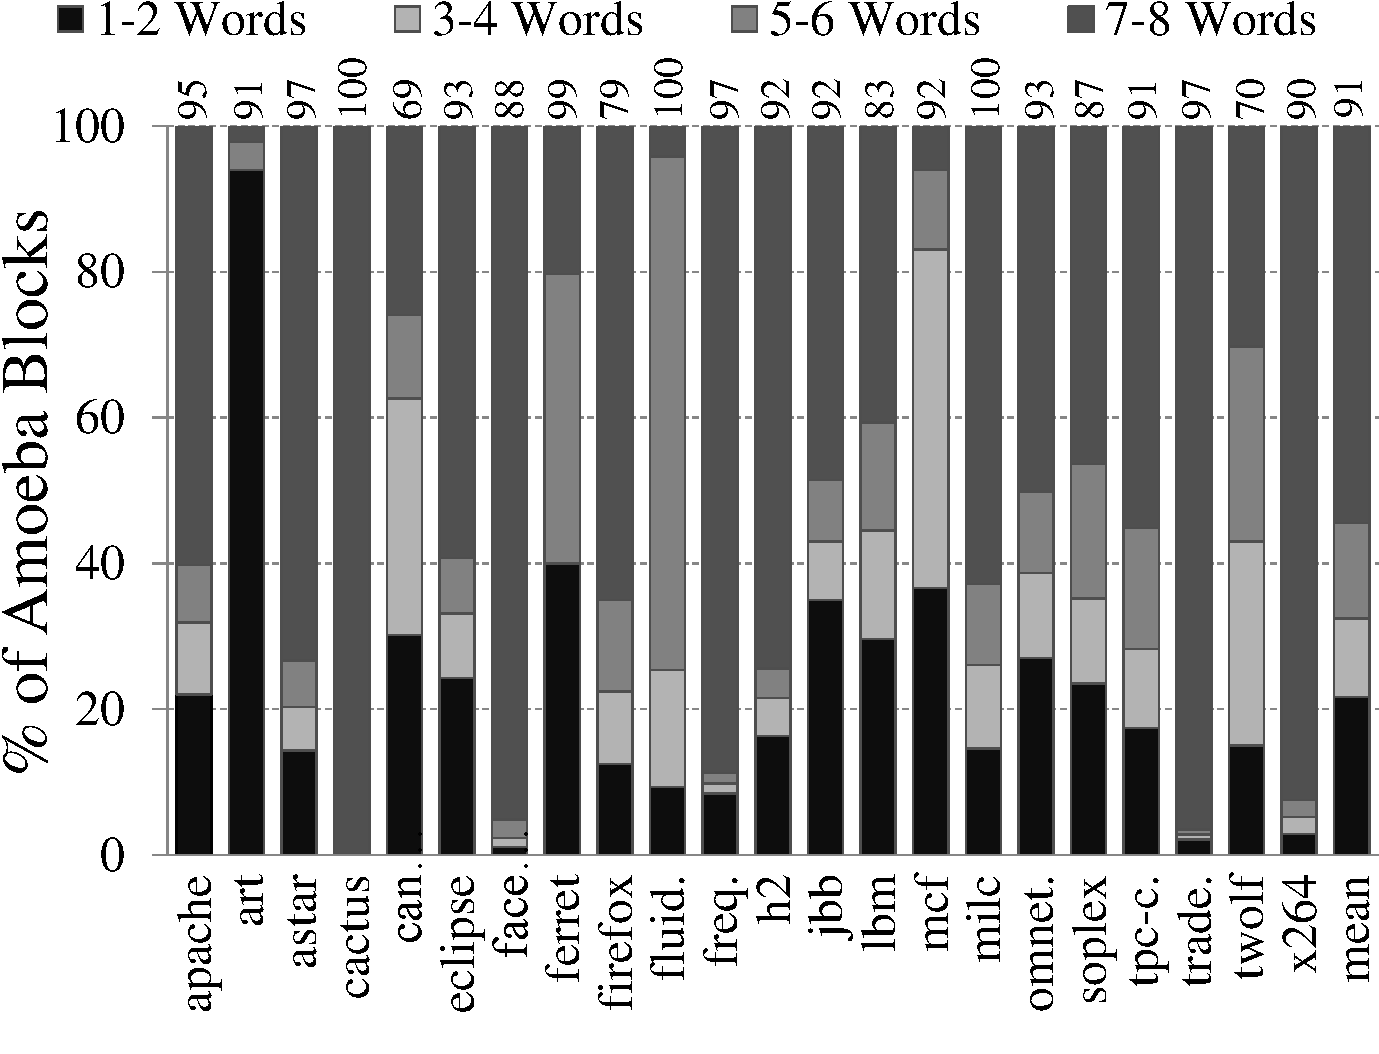
\includegraphics[width=0.8\textwidth]{files/Plots/08-StackBar_PredictSize_1M.pdf}
  }
  \caption[Distribution of cache block sizes]{Distribution of cache line granularities in the (a) 64K L1 and (b) 1M L2 \AC{}. Average utilization is on top.}
  \label{fig:StackBar_PredictorSize}
\end{figure}

\clearpage

\begin{figure}[!h]
  \centering
  \subfloat[64K L1 cache]{
    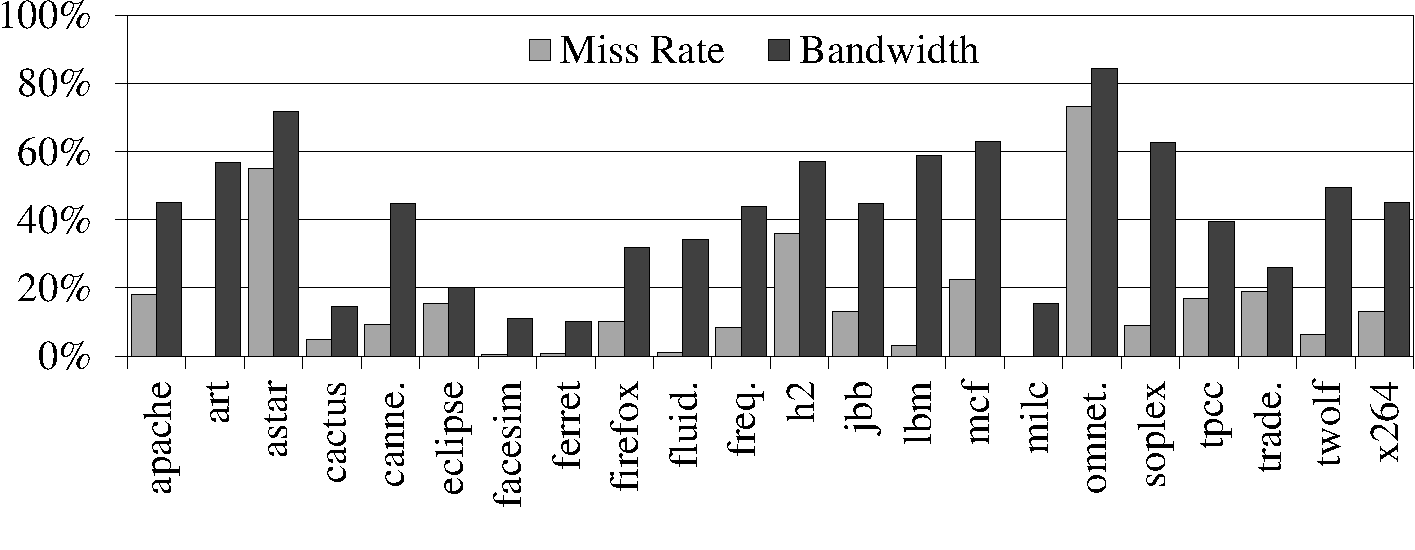
\includegraphics[width=\textwidth]{files/Plots/08-Oracle-64K-Miss-BW-Improvement.pdf}
  }

  \subfloat[1M L2 cache]{
    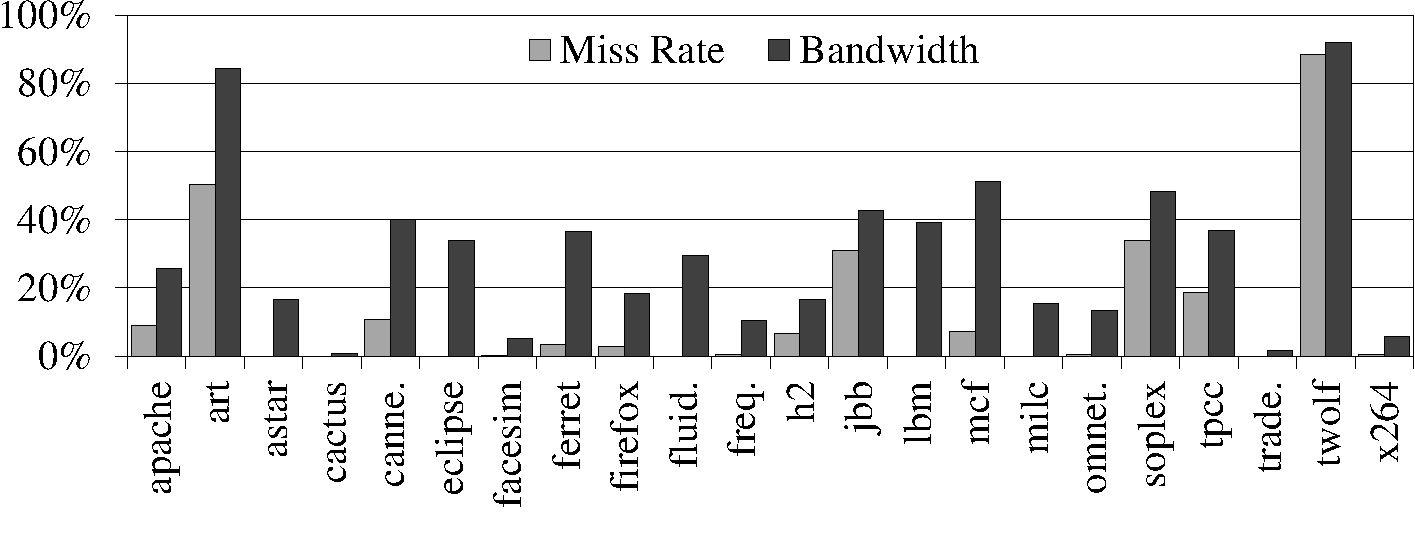
\includegraphics[width=\textwidth]{files/Plots/08-Oracle-1M-Miss-BW-Improvement.pdf}
  }
  \caption[Miss Rate and Bandwidth Improvement]{Miss Rate and bandwidth reduction with respect to a fixed granularity conventional cache with cache line size 64 bytes for (a) 64K equivalent \AC\ and (b) 1M equivalent \AC{}.}
  \label{fig:miss_bw_reduction}
\end{figure}

\section{Overall Performance and Energy}
\label{sec:overall_performance_and_energy}
\noindent \textbf{Result 3:}{~\AC\ improves overall cache efficiency and boosts performance by 10\% on commercial applications\footnote{``Commercial'' applications includes Apache, SpecJBB and TPC-C.}, saving up to 11\% of the energy of the on-chip memory hierarchy. Off-chip L2$\leftrightarrow$memory energy sees a mean reduction of 41\% across all workloads. 

\begin{figure}[!h]
  \centering
    \subfloat[Energy Improvement]{
      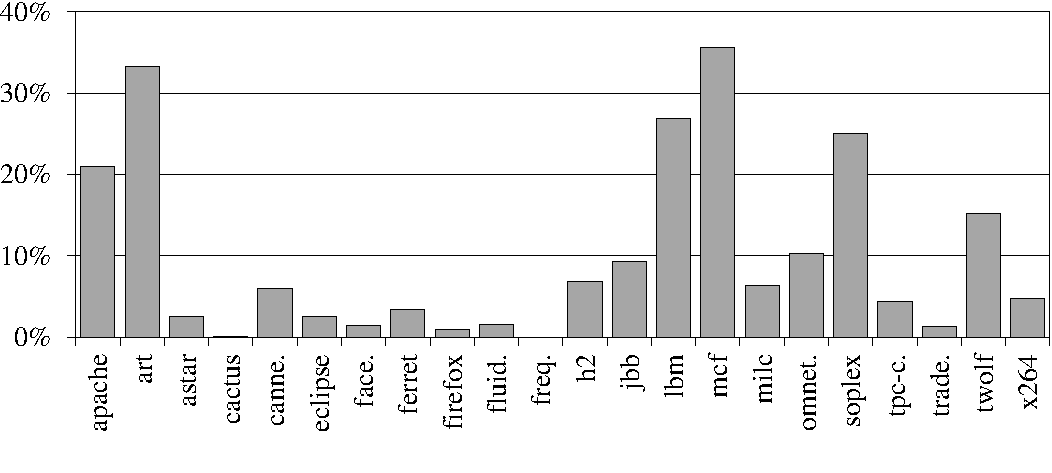
\includegraphics[width=\textwidth]{files/Plots/08-Oracle_Energy.pdf}
    }
    
    \subfloat[Performance Improvement]{
      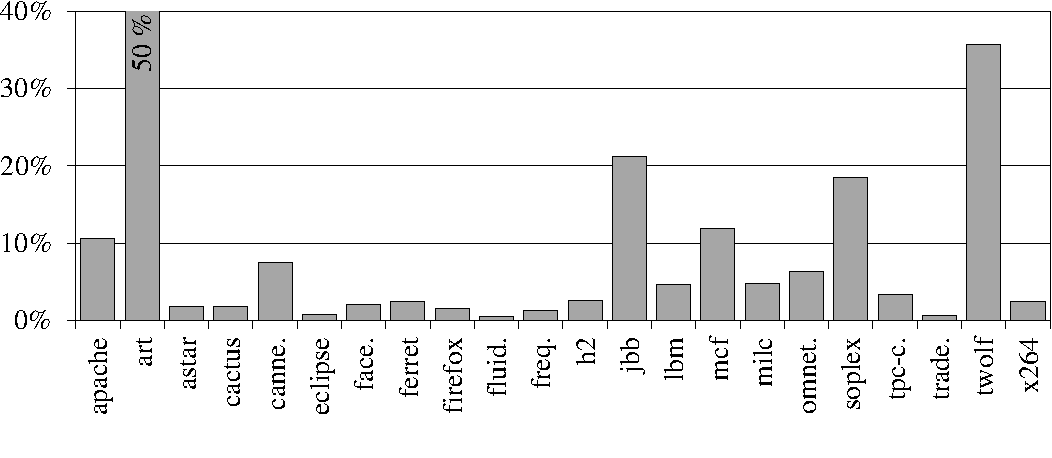
\includegraphics[width=\textwidth]{files/Plots/08-Oracle_Perf.pdf}
    }
    \caption{ The above charts (a) show the percentage reduction in energy and (b) the percentage reduction in cycle time for an \AC\ compared to a fixed granularity conventional cache with 64K L1 and 1M LLC. Higher bars indicate better performance. Y-axis terminated to illustrate bars clearly.}
    \label{plot:multi_sys_perf_energy}
\end{figure}

\clearpage

A two-level cache hierarchy is modeled in which the L1 is a 64K cache with 256 sets (3 cycles load-to-use) and the L2 is 1M, 8192 sets (20 cycles). A fixed memory latency of 300 cycles is assumed. It is assumed that the L1 access is the critical pipeline stage and throttle CPU clock by 4\% (an alternative approach is evaluated in the next section).  The total dynamic energy of the \AC\ is calculated using the energy numbers determined in Section~\ref{sec:area_latency_energy_overhead} through a combination of synthesis and CACTI~\cite{Muralimanohar:2007:ONO:1331699.1331704}. 4 fast tags per set at the L1 and 8 fast tags per set at the L2 are used. The penalty for all the extra metadata in the \AC{} is included. The energy for a single L1---L2 transfer (6.8pJ per byte) is derived from~\cite{weti,Muralimanohar:2007:ONO:1331699.1331704}. The interconnect uses full-swing wires at 32nm, 0.6V. 

Figure~\ref{plot:multi_sys_perf_energy} plots the overall improvement in performance and reduction in on-chip memory hierarchy energy (L1 and L2 caches, and L1$\leftrightarrow$L2 interconnect). For applications that have good spatial locality (e.g., tradesoap, milc, facesim, eclipse, and cactus), the \AC\ has minimal impact on miss rate, but provides significant benefit in terms of reduction in bandwidth. This results in on-chip energy reduction: milc's L1$\leftrightarrow$L2 bandwidth reduces by $\simeq$15\%(see Figure~\ref{fig:miss_bw_reduction}(a)) and its on-chip energy reduces by 5\%. Applications that suffer from cache pollution under \textit{Fixed} (apache, jbb, twolf, soplex and art) see gains in performance and energy. Apache's performance improves by 11\% and on-chip energy reduces by 21\%, while SpecJBB's performance improves by 21\% and energy reduces by 9\%. Art gains approximately 50\% in performance.  Streaming applications like mcf access blocks with both low and high utilization. Keeping out the unused words in the under-utilized blocks prevents the well-utilized cache blocks from being evicted; mcf's performance improves by 12\% and on-chip energy by 36\%.

\subsection{Extra cache pipeline stage}
\label{sec:extra_cache_pipeline_stage}

An alternative strategy to accommodate \AC{}'s overheads is to add an extra pipeline stage to the cache access which increases hit latency by 1 cycle. The CPU clock frequency entails no extra penalty compared to a conventional cache. Using such a design, applications in the moderate and low spatial locality group (8 applications), the \AC\ continues to provide a performance benefit between 6---50\%. milc and canneal suffer minimal impact, with a 0.4\% improvement and 3\% slowdown respectively.  Applications in the high spatial locality group (12 applications) suffer an average 15\% slowdown (maximum 22\%) due to the increase in L1 access latency. In these applications, 43\% of the instructions (on average) are memory accesses and a 33\% increase in L1 hit latency imposes a high penalty. Note that all applications continue to retain the energy benefit. The cache hierarchy energy is dominated by the interconnects and the \AC\ provides notable bandwidth reduction. While these results may change for an out-of-order, multiple-issue processor, the evaluation suggests that \AC\ if implemented with the extra pipeline stage is more suited for lower levels in the memory hierarchy than the L1.  

\begin{figure}[h]
  \centering
  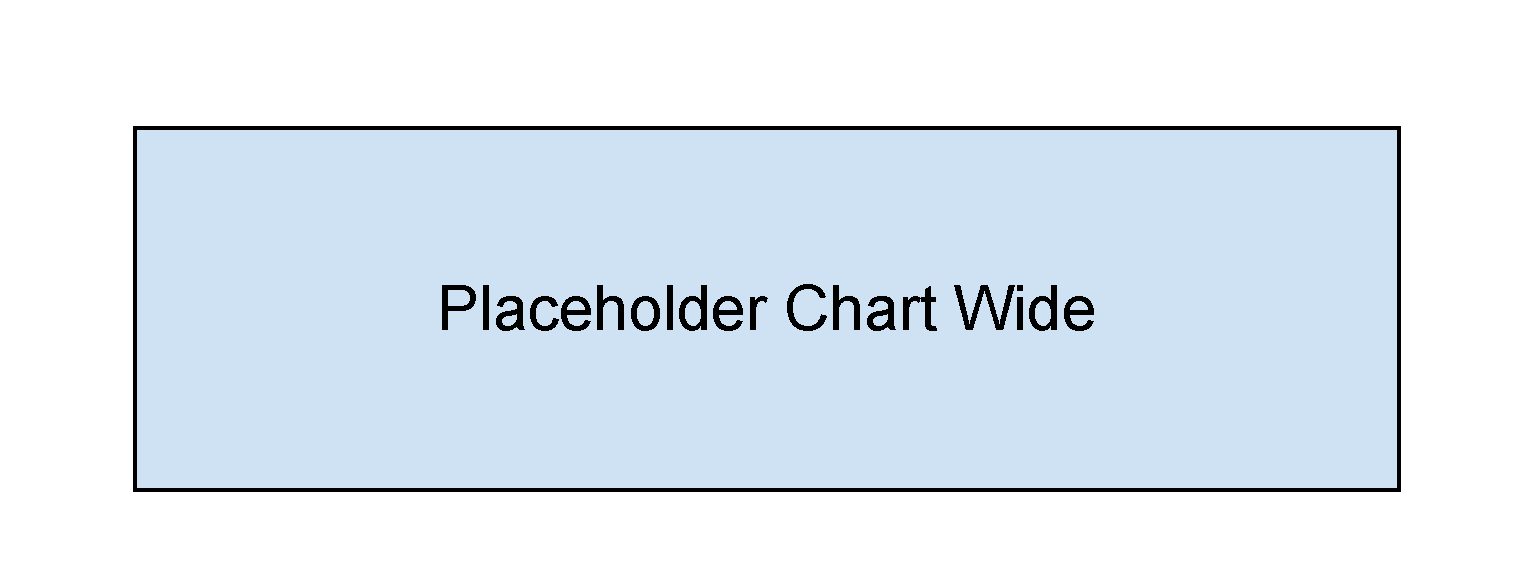
\includegraphics[width=\textwidth]{files/Figures/Placeholder_Chart_Wide.pdf}
  \caption{Placeholder for extra pipeline stage performance plot -- all apps}
  \label{fig:extra_cache_pipeline_stage}
\end{figure}

\subsection{Off-chip L2$\leftrightarrow$Memory energy}
The L2's higher cache capacity makes it less susceptible to pollution and provides less opportunity for improving miss rate. In such cases, the \AC\ keeps out unused words and reduces off-chip bandwidth and thereby off-chip energy. We assume that the off-chip DRAM can provide adaptive granularity transfers for \AC{}'s L2 refills as in~\cite{Yoon_Jeong_Erez_2011}. The DRAM model used was presented in a recent study~\cite{exascale} and consumes 0.5nJ per word transferred off-chip. The low spatial locality applications see a dramatic reduction in off-chip energy. For example, twolf sees a 93\% reduction. On commercial workloads the off-chip energy decreases by 31\% and 24\% respectively. Even for applications with high cache utilization, off-chip energy decreases by 15\%.

\begin{figure}[h]
  \centering
  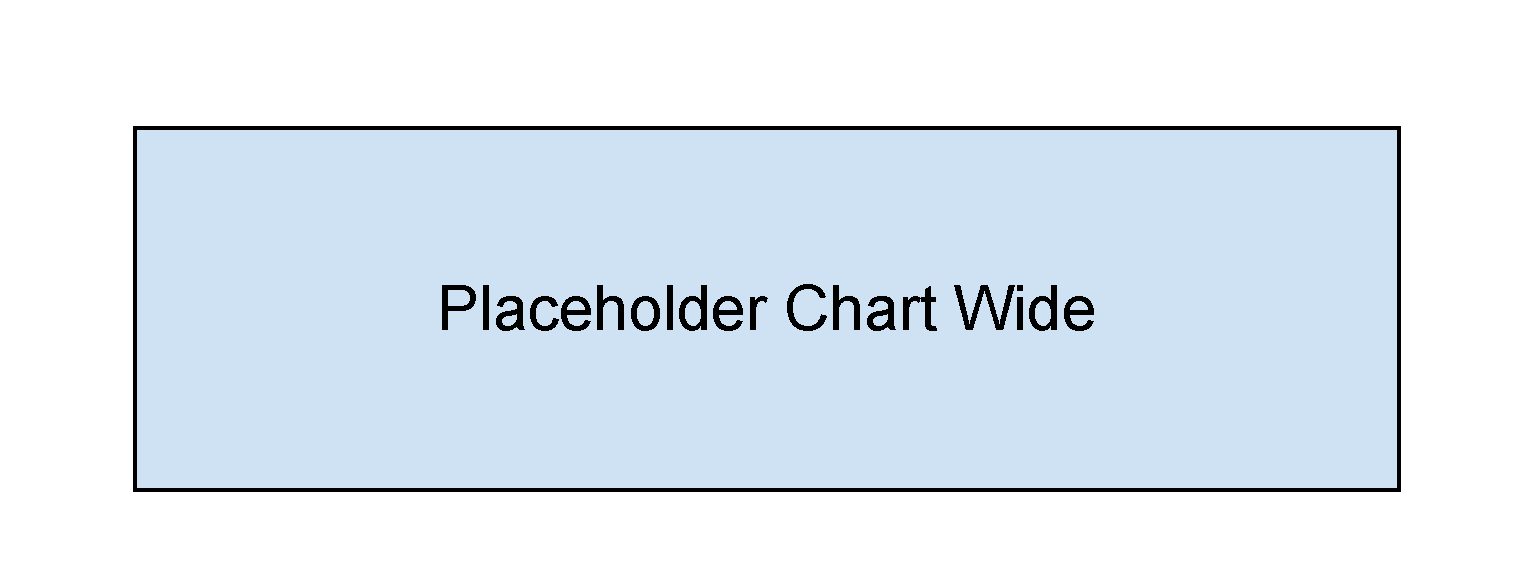
\includegraphics[width=\textwidth]{files/Figures/Placeholder_Chart_Wide.pdf}
  \caption{Placeholder for off chip energy plot -- all apps}
  \label{fig:offchip_energy}
\end{figure}


\section{Spatial Predictor Tradeoffs}
\label{sec:spatial_predictor_tradeoffs}

The effectiveness of spatial pattern prediction is evaluated in this section. In the table-based approach, a pattern history table records spatial patterns from evicted blocks and is accessed using a prediction index. The table-driven approach requires careful consideration of the following: prediction index, predictor table size and training period. The effects are quantified by comparing the predictor against a baseline fixed-granularity cache. A baseline 64K cache is used since it induces enough misses and evictions to highlight the predictor tradeoffs clearly.

\subsection{Predictor Indexing} 

A critical choice with the history-based prediction is the selection of the predictor index. Two types of predictor indexing were explored:
\begin{itemize}[noitemsep]
  \item a program counter based(\code{PC}) approach\cite{chen-hpca-2004} based on the intuition that fields in a data structure are accessed by specific PCs and tend to exhibit similar spatial behavior. The tag includes the PC and the critical word index: $((PC>>3)<<3)+\frac{(addr\%64)}{8}$.
  \item a \textit{Region}-based (\code{REGION}) approach that is based on the intuition that similar data objects tend to be allocated in contiguous  regions of the address space and tend to exhibit similar spatial behavior. 
\end{itemize}

The miss rate and bandwidth properties of both the  \code{PC} (256 entries, fully associative) and \code{REGION} (1024 entries, 4KB region size) predictors were compared. The size of the table used in each predictor was selected as the optimal found by empirical analysis for each predictor type.  For all applications apart from cactus (a high spatial locality application), \code{REGION}-based prediction tends to overfetch and waste bandwidth as compared to \code{PC}-based prediction, which has 27\% less bandwidth consumption on average across all applications. For 17 out of 22 applications, \code{REGION}-based prediction shows 17\%  better MPKI on average (max: 49\% for cactus). For 5 applications (apache, art, mcf, lbm, and omnetpp), \code{PC} has better accuracy when predicting the spatial behavior of cache blocks than \code{REGION} and demonstrates a 24\% improvement in MPKI (max: 68\% for omnetpp).

\subsection{Predictor Table}

The organization and size of the pattern table was studied using the \code{REGION} predictor. The following parameters were evaluated :
\begin{itemize}[noitemsep]
  \item region size, which directly correlates with the coverage of a fixed-size table
  \item the size of the predictor table
  \item the number of bits required to represent the spatial pattern.
\end{itemize}

Large region sizes effectively reduce the number of regions in the working set and require a smaller predictor table. However, a larger region is likely to have more blocks that exhibit varied spatial behavior and may pollute the pattern entry.  We find that going from 1KB (4096 entries) to 4KB (1024 entries) regions, the 4KB region granularity decreased miss rate by 0.3\% and increased bandwidth by 0.4\% even though both tables provide the same working set coverage (4MB).  Fixing the region size at 4KB, we studied the benefits of an unbounded table.  Compared to a 1024 entry table (\code{FINITE} in Figure~\ref{fig:Predictor_All_Apps}), the unbounded table increases miss rate by 1\% and decreases bandwidth by 0.3\% . A 1024 entry predictor table (4KB region granularity per-entry) suffices for most applications. Organizing the 1024 entries as a 128-set$\times$8-way table sufficesfor eliminating associativity related conflicts ($<$0.8\% evictions due to lack of ways).

Focusing on the number of bits required to represent the pattern table, we evaluated the use of 4-bit saturation counters (instead of 1-bit bitmaps). The saturation counters seek to avoid pattern pollution when blocks with varied spatial behavior reside in the same region. Interestingly, we find that it is more beneficial to use 1-bit bitmaps for the majority of the applications (12 out of 22); the hysteresis introduced by the counters increases training period.  

To summarize, we find that a \code{REGION} predictor with region size 4KB and 1024 entries can predict the spatial pattern in a majority of the applications. CACTI indicates that the predictor table can be indexed in 0.025ns and requires 2.3pJ per miss indexing.

\subsection{Spatial Pattern Training} 

A widely-used approach to training the predictor is to harvest the word usage information on an eviction. Unfortunately, evictions may not be frequent, which means the predictor's training period tends to be long, during which the cache performs less efficiently and/or that the application's phase has changed in the meantime. Particularly at the time of first touch (compulsory miss to a location), we need to infer the global spatial access patterns. We compare the finite region predictor (\code{FINITE} in Figure~\ref{fig:Predictor_All_Apps}) that only predicts using eviction history, against a \code{FINITE+FT}: this adds the optimization of inferring the default pattern (in this paper, from a prior run) when there is no predictor information. \code{FINITE+FT} demonstrates an avg. 1\% (max: 6\% for jbb) reduction in miss rate compared to \code{FINITE} and comes within 16\% the miss rate of \code{HISTORY}. In terms of bandwidth \code{FINITE+FT} can save 8\% of the bandwidth (up to 32\% for lbm) compared to \code{FINITE}. The percentage of first-touch accesses is shown in Table~\ref{table:Abs_Eval_Oracle}.  

% Maybe we should point out that the first touch is a more important
% optimisation for bandwidth as our fall back was to predict a full cache line
% which would have not have a first order impact on miss rate.

\begin{figure}[h]
  \centering
    \subfloat[Misses Per Kilo Instructions]{
      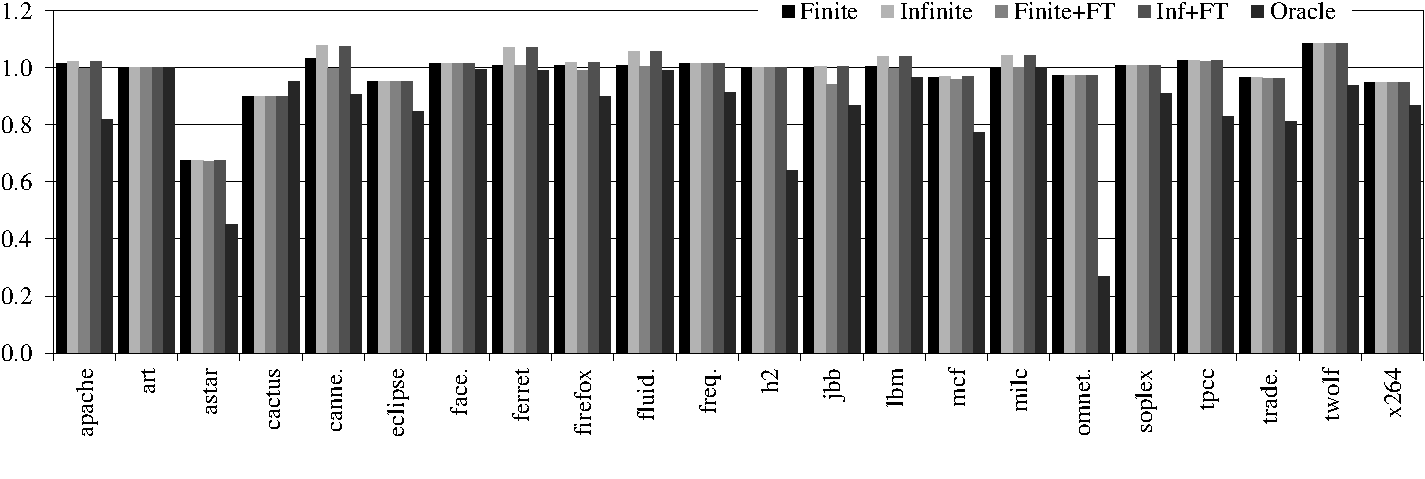
\includegraphics[width=\textwidth]{files/Plots/08-Predictor-MPKI.pdf}
    }
    
    \subfloat[Bandwidth]{
      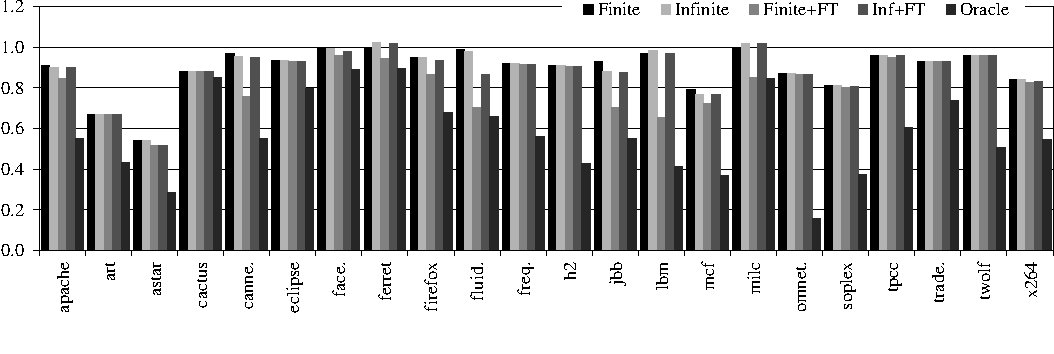
\includegraphics[width=\textwidth]{files/Plots/08-Predictor-BW.pdf}
    }
    \caption[Predictor Performance]{ The charts above show the performance of the different types of \AC\ predictors in terms of misses per kilo instructions and miss bandwidth for a 64K L1 equivalent scaled to the performance of a fixed granularity conventional cache. \\ \\
      \code{FINITE}: \code{REGION} predictor (1024 entry table and 4K region size). \\
      \code{INFINITE}: Unbounded predictor table (\code{REGION} predictor). \\ 
      \code{FINITE+FT}: \code{FINITE} with hints for prediction on compulsory misses (first touches). \\
      \code{INF+FT}: \code{INFINITE} with hints for prediction on compulsory misses (first touches). \\
      \code{HISTORY}: Uses spatial pattern hints collected at eviction from a prior run. 
    }
    \label{fig:Predictor_All_Apps}
\end{figure}

\clearpage

\subsection{Predictor Summary}
\begin{itemize}
  \item For the majority of the applications (17/22) the address-region predictor with region size 4KB works well. However, five applications (apache, lbm, mcf, art, omnetpp) show better performance with PC-based indexing. For best efficiency, the predictor should adapt indexing to each application. 
  \item Updating the predictor only on evictions leads to long training periods, which causes loss in caching efficiency. We need to develop mechanisms to infer the default pattern based on global behavior demonstrated by resident cache lines.
  \item The online predictor reduces MPKI by 7\% and bandwidth by 26\% on average relative to the conventional approach. However, it still has a 14\% higher MPKI and 38\% higher bandwidth relative to the \code{HISTORY}-based predictor, indicating room for improvement in prediction. 
  \item The 1024-entry (4K region size) predictor table imposes $\simeq$0.12\% energy overhead on the overall cache hierarchy energy since it is referenced only on misses.
\end{itemize}

\section{\AC\ Adaptivity}
\label{sec:adaptivity}

We demonstrate that \AC{} can adapt better than a conventional cache to the variations in spatial locality.

\subsection{Tuning RMAX for High Spatial Locality} 

A challenge often faced by conventional caches is the desire to widen the cache block (to achieve spatial prefetching) without wasting space and bandwidth in low spatial locality applications. We study 3 specific applications: milc and tradesoap have good spatial locality and soplex has poor spatial locality. With a conventional 1M cache, when we widen the block size from 64 to 128 bytes, milc and tradesoap experience a 37\% and 39\% reduction in miss rate. However, soplex's miss rate increases by 2$\times$ and bandwidth by 3.1$\times$.

With \AC\, we do not have to make this uneasy choice as it permits \AB{}s with granularity 1---RMAX words (RMAX: maximum block size). When we increase RMAX from 64 bytes to 128 bytes, miss rate reduces by 37\% for milc and 24\% for tradesoap, while simultaneously lowering bandwidth by 7\%. Unlike the conventional cache, \AC\ is able to adapt to poor spatial locality: soplex experiences only a 2\% increase in bandwidth and 40\% increase in miss rate.

\begin{figure}[!ht]
  \centering
  \vspace{10pt}
  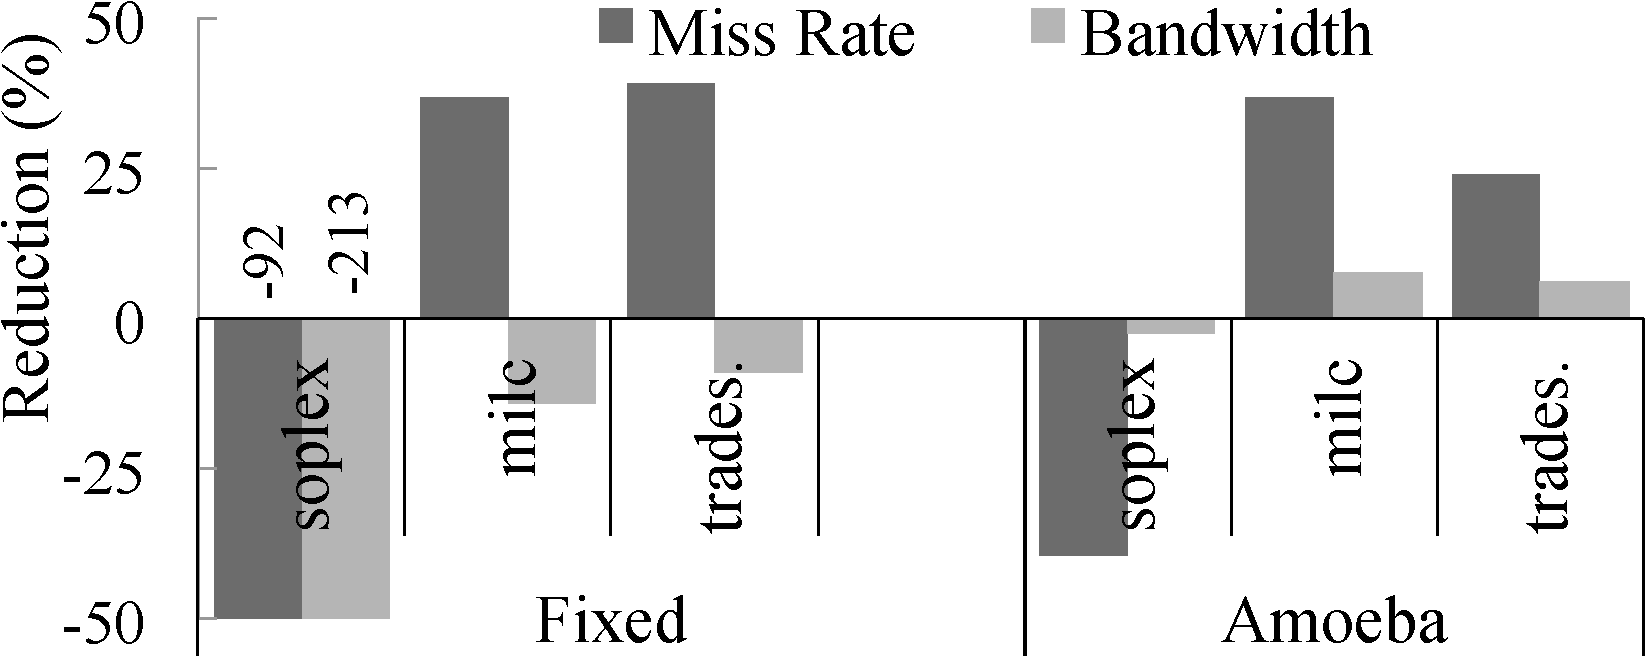
\includegraphics[width=0.7\textwidth]{files/Plots/08-Bar-Fixed-RMAX.pdf}
  \label{fig:rmax}
  \caption{Effect of increase in block size from 64 to 128 bytes in a 1 MB cache}
 
\end{figure}

\subsection{Predicting Strided Accesses} 
Many applications (e.g.,firefox and canneal) exhibit strided access patterns, which touch a few words in a block before accessing another block. Strided accesses patterns introduce intra-block holes (untouched words). For instance, canneal accesses $\simeq$10K distinct fixed granularity cache blocks  with a specific access pattern, \textbf{[{-}{-}x{-}{-}x{-}{-}]} (\textbf{x} indicates $i^{th}$ word has been touched). 

%!TEX root=/home/ska124/Dropbox/Thesis/thes-full.tex
\begin{table}[!htb]
  \centering
  \begin{tabular}{|l|c|c|c|c| }
    \hline
    & \multicolumn{2}{c|}{canneal} &  \multicolumn{2}{c|}{firefox} \\
    \hline
    & Miss Rate & BW & Miss Rate & BW\\
    \hline
    Policy-Miss & 10.31\% & 81.2\% & 11.18\% & 47.1\%\\
    \hline
    Policy-BW & --20.08\% & 88.09\% & --13.44\% & 56.82\%\\
    \hline
    Spatial Patterns & \multicolumn{2}{c|}{\textbf{[{-}{-}x{-}{-}x{-}{-}]
        [x{-}{-}x{-}{-}{-}{-}]}} &
    \multicolumn{2}{c|}{\textbf{[{-}x{-}{-}x{-}{-}{-}]
        [x{-}{-}{-}x{-}{-}{-}]}} \\
    \hline
    \multicolumn{4}{c}{--: indicates Miss or BW higher than Fixed.}
  \end{tabular}
  \caption{Predictor Policy Comparison}
  \label{table:predictor_policy}
\end{table}

Any predictor that uses the access pattern history has two choices when an access misses on word 3 or 6 a) A miss oriented policy (Policy-Miss) may refill the entire range of words 3--6 and eliminate the secondary miss but bring in untouched words 4--5, increasing bandwidth, and b) a bandwidth focused choice (Policy- BW) that refills only the requested word but will incur more misses. Table~\ref{table:predictor_policy} compares the two contrasting policies for \AC{} (relative to a Fixed granularity baseline cache). Policy-BW saves 9\% bandwidth compared to Policy-Miss but suffer 25-30\% higher miss rate.

%!TEX root=/home/ska124/Dropbox/Thesis/thes-full.tex
\begin{table}[h]
\centering
	\begin{tabular}{|c|c|c|c|c|c|c|c|c|}
	\hline
	 & \multicolumn{2}{c|}{MPKI} &  \multicolumn{2}{c|}{BW Bytes/1K} & CPI & \multicolumn{2}{c|}{Predictor Stats}  \\
	\hline
	          & L1        & L2    & L1$\longleftrightarrow$L2 & L2$\longleftrightarrow$Mem & & FT &  \\
	          & MPKI & MPKI & Bytes/1K & Bytes/1K & Cycles/Ins. & Miss \% &  Ins/Evict\\
	\hline
	apache    &    64.9 & 19.6    &    5,000  &    2,067         &  8.3  & 0.4 &   17 \\
	art       &    133.7  &    53.0    &    5,475  &    1,425    &  16.0 & 0.0 &   9 \\
	astar     &    0.9    &    0.3     &    70     &    35       &  1.9  & 18.0 &  1,600 \\
	cactus    &    6.9    &    4.4     &    604    &    456      &  3.5  & 7.5 &   162 \\
	canne.    &    8.3    &    5.0     &    486    &    357      &  3.2  & 5.8 &   128 \\
	eclip.    &    3.6    &    $<$0.1  &    433    &    $<$1     &  1.8  & 0.1 &   198 \\
	faces.    &    5.5    &    4.7     &    683    &    632      &  3.0  & 41.2 &  190 \\
	ferre.    &    6.8    &    1.4     &    827    &    83       &  2.1  & 1.3 &   156 \\
	firef.    &    1.5    &    1.0     &    123    &    95       &  2.1  & 11.1 &  727 \\
	fluid.    &    1.7    &    1.4     &    138    &    127      &  1.9  & 39.2 &  629 \\
	freqm.    &    1.1    &    0.6     &    89     &    65       &  2.3  & 17.7 &  994 \\
	h2        &    4.6    &    0.4     &    328    &    46       &  1.8  & 1.7 &   154 \\
	jbb       &    24.6   &    9.6     &    1,542  &    830      &  5.0  & 10.2 &  42 \\
	lbm       &    63.1   &    42.2    &    3,755  &    3,438    &  13.6 & 6.7 &   18 \\
	mcf       &    55.8   &    40.7    &    2,519  &    2,073    &  13.2 & 0.0 &   19 \\
	milc      &    16.1   &    16.0    &    1,486  &    1,476    &  6.0  & 2.4 &   66 \\
	omnet.    &    2.5    &    $<$0.1  &    158    &    $<$1     &  1.9  & 0.0 &   458 \\
	sople.    &    30.7   &    4.0     &    1,045  &    292      &  3.1  & 0.9 &   35 \\
	tpcc      &    5.4    &    0.5     &    438    &    36       &  2.0  & 0.4 &   200 \\
	trade.    &    3.6    &    $<$0.1  &    410    &    6        &  1.8  & 0.6 &   194 \\
	twolf     &    23.3   &    0.6     &    1,326  &    45       &  2.2  & 0.0 &   49 \\
	x264      &    4.1    &    1.8     &    270    &    190      &  2.2  & 12.4 &  274 \\
	\hline                                  
	\end{tabular}                                                                       
                                                                       
\caption[Absolute performance statistics]{Abslute performance statistics for the \AC\ using a \code{Region} predictor(infinite table size) with predictions for compulsory misses serviced using data collected from a prior run of the application. Higher value for Ins/Evict indicates predictor training takes longer. \\ \\
	\textbf{MPKI} : Misses / 1K instructions. \\
	\textbf{BW}: Number of words / 1K instructions. \\
	\textbf{CPI}: Clock cycles per instruction. \\
	\textbf{FT}: Percentage of misses that are compulsory misses.  \\
	\textbf{Ins/Evict}: Number of instructions between evictions. 
}
\label{table:Abs_Eval_Oracle}                                        
\end{table}                                                          
\clearpage

% First Touch info for Inf Table
% 0.4
% 0.0
% 18.0
% 7.5
% 5.8
% 0.1
% 41.2
% 1.3
% 11.1
% 39.2
% 17.7
% 1.7
% 10.2
% 6.7
% 0.0
% 2.4
% 0.0
% 0.9
% 0.4
% 0.6
% 0.0
% 12.4

% First Touch info for 1K Table
% 16.0
% 0.0
% 20.1
% 9.5
% 44.0
% 0.1
% 76.3
% 20.1
% 44.9
% 86.6
% 19.3
% 2.7
% 55.4
% 57.0
% 13.6
% 93.2
% 0.0
% 1.9
% 5.1
% 0.6
% 0.0
% 19.0


% Instructions per Eviction data for Oracle 64K

% 17
% 9
% 1,600
% 162
% 128
% 198
% 190
% 156
% 727
% 629
% 994
% 154
% 42
% 18
% 19
% 66
% 458
% 35
% 200
% 194
% 49
% 274